\documentclass{article}
\usepackage{gensymb}
\usepackage{graphicx}
\graphicspath{ {./res-images/} }
\usepackage{listings}
\begin{document}

\title{Building Resilience Vaccine Distribution}
\author{Saransh Sharma }
\date{January 2021}


\maketitle


\abstract

The COVID-19 pandemic has been one of the most influential pandemics in a century. Conventional life has been disrupted on a global scale, with rampant disease transmission leading to an unusual number of deaths. To take measures for this widespread virus transmission, vaccines have been developed since the early emergence of the pandemic. However, due to the substantial burden on the medical community and the gradual collapse of economies worldwide, vaccine testing processes were expedited to stabilize the uncontrolled virus. Development of some vaccines was accelerated by combining multiple phases of vaccine testing by running them in parallel. Once developed, the vaccines received early or limited approval. Yet, the distribution infrastructure and strategies remain undetermined, especially in necessitous regions. This study aims to address some of the deficiencies in the administration and distribution infrastructure of vaccines while proposing efficient and systematized strategies. 

\section{Introduction}

Vaccine in India is approved for restricted use in emergency situation in public interest as an abundant precaution, in clinical trial mode, especially in the context of infection by mutant strains.\footnote{https://www.bbc.com/news/world-asia-india-55534902}, though there are serious concerns on lack of evidence and unsatisfactory scientific evidence for the vaccine produced in India.\footnote{bae2020challenges}

Planning for country wide operations has already begun, for now frontline workers and people in need like age above 50 with pre-conditions will receive vaccine first. Current situation of infection across globe stands at 37.3 M, 10M+ in India. COVID-19 amounts to 149K death in India alone.
Government of India has launched COWIN program\footnote{https://pib.gov.in/PressReleasePage.aspx?PRID=1683001} to strengthen vaccine intelligence, this open call is for partners to provide answers to 7 key problems identified by government.

Before building a strong vaccine intelligence network that provides last mile delivery to the one in need there needs a strong focus on filling the gaps in distribution. The world’s manufacturing processes and supply chains are underprepared for the task of widespread vaccine distribution\cite{bae2020challenges}.Movement of vaccine in India posses challenges of unknown and unresolved issues that can cause delay. To be able to implement at scale key challenges of maintaining stable temperature ie cold chain , current capacity of cold chain is inadequate for existing vaccination programs\footnote{https://www.bloombergquint.com/global-economics/india-faces-cold-chain-logistics-challenge-for-virus-vaccination}. WHO recommends vaccine should be stored at 2-8\degree C, but studies showing vaccines are exposed to temperature above 8 \degree C\cite{dhere2011pandemic} at every level of storage as vaccine cross different regions. Hence, Coordinated efforts between regional level needed to achieve a stable cold chain with an alternative approach that can offset the waste of vaccine.

Recording data at sites of users by healthcare worker is critical, studies has shown that 10-60\% of data is inaccurate\cite{atkinson2020digital}. Several challenges like what kind of data is recorded when administering vaccine still persist. Finding solutions and alternative interfaces to record data to reduce inaccuracy. Utilising that data for managing validation across the information system. Data management across different level of local, regional and state. This data could be used across different verticals to make descions.

In this paper we define different approaches and practical solutions to certain problems we have identified by reviwing literature. We have defined these solutions in 

\begin{itemize}
	\item Synchronicity
	\item Event Layer
	\item AI For Finding Locations
	\item Cold Chain Alternative
	\item Use of Cryptographic Methods
\end{itemize}




\section{Synchronicity}
In order to capture and utilise data from different verticals it is important to implement synchronous data layer that keeps updating data in real time. There are going to be variety of services that is going to create data attributes. A service that interacts with VIN sends a message , that passes through a parser and goes to the receiving end. This whole process can be stored as message streams or log for various auditable purpose later. This process is known as event sourcing , services recording all the states together as a sequence of events, this kind of design allow to reconstruct past states. Its quite straightforward and less consuming than querying database.

Implementing an indexer that identifies what kind of attributes are most frequently used , those attributes can be stored as meta-data. This meta-data can be used as a template when a service is sending out a message. For an eg: At a clinic when frontline worker recording data about vaccine, they could use the metadata rather then pre-defined field. This meta-data is useful in terms of what kind of attributes is important from different verticals.

General steps of the building a sync layer is to have a Parser, the job of a parser is to clean data, after messages gets through parser validating data. The major goal of this layer is to reduce friction and establish communication between working groups and services.

Practical Application such as RFID, sensors, Applications collecting data from delivery points, logistics and supply chain instrument that will create data at different vectors.

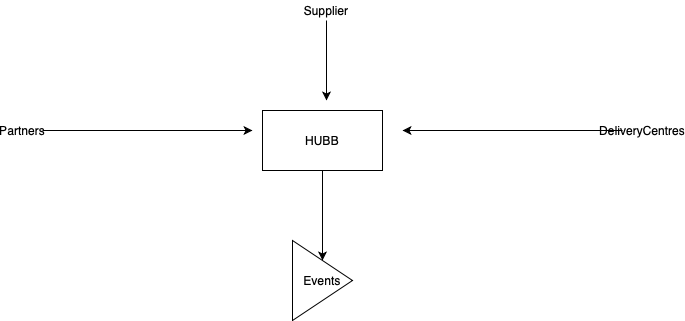
\includegraphics[scale=0.5]{hubb}


\begin{lstlisting}
	createData()
	parseData()
	processData()
		identify()
		extract()
		reshape()
	return()	
\end{lstlisting}

   
\section{Eventing Layer}

A process that involves sending out important alerts and notices	, eventing layer comes in place. The overall use of  layer is to identify and sends notices and warnings to the interested parties and services that are involved in a process. A process could be like delivering vaccines to users, shipping vaccines from a location. All of these processes have pre-defined steps and in case of deviation of these step eventing layer should send out notifications to involved parties.

One example is to use this service to manage end to end shipping and defining events points, these points can be flow, or logical steps, or an incident. When any incident is triggered at any level, parties are notified. Practical example, vaccine supply reaches with tampered unit, notices and alerts reaching to vaccine delivery site and the one who delivered.

This eventing layer can use the above data layer to identify parameters from data attributes, like when to send notification, who to send like who are parties. This kind of eventing layer is already available in modern web-apps these days specifically in machine learning.

\section{AI}
AI is a powerful catalyst today, the use of AI in healthcare is quite visible such as  drug discovery. Scientist are using inexpensive and rapid implementation for finding therapies, if given enough data it can aid the search of the drug\cite{keshavarzi2020artificial}. Once we have built the information that allow us to have quality data with few errors, we could use sophisticated math models and to train them using re-inforcement learning. Hence machine could be trained and  help in predictions for forecasting inventory, preparing for hazard , analysing the turn around time based on the overall supply chain optimal functioning. We describe these models here that can be fed in any application to achieve optimal distribution.

\begin{enumerate}
	\item Present vaccine distribution largely focus on individual at risk, We can use spatiotemporal regions with the most new cases of infection during a certain time frame and compare it with the standard practice of distributing vaccines demographically. A computational model presented in\cite{grauer2020strategic} , for a locally well-mixed population,strongly reduces the number of deaths by 35\%. This model purely puts emphasis on density of the population on a given space and time ie a region, targeting using a math based model and realising herd immunity.
	\item Typically vaccines are distributed via a four-tier hierarchical networks, classic WHO-EPI model inherently is limited to meeting the demand, fixing location of the clinic. Mixed integer programming solves key issues of selecting storage sizes and ensures all delivery is made in single trip\cite{yang2020optimizing}. This model is based on hubs, nodes associated to these hubs. Below table shows the numerical output using MIP model.
  
	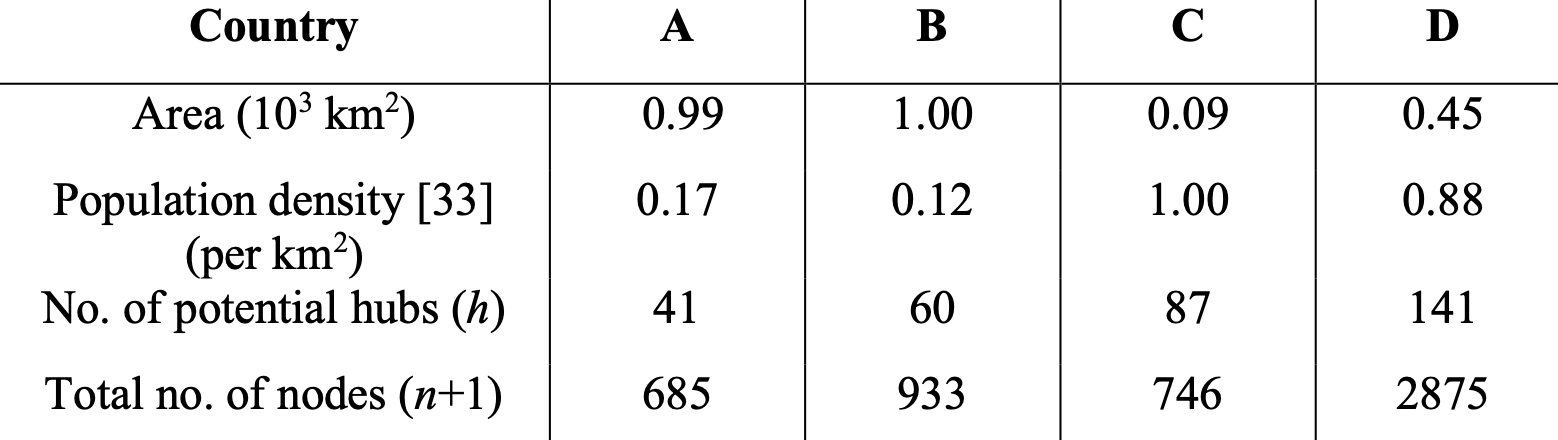
\includegraphics[scale=0.4]{maths.png}
	\item Since real world experimentation is out of question , there are unknown problems that can occur, scarcity of vaccine or sub-components. Resulting dynamics may change over time, enough data supplied with contextual policies with demographics for the fair distribution. VacSim model emphasis challenges that need solving in real time, with no ground truth availability. This model employs classic re-inforcement learning with forward feed that can be optimised in real time.\cite{awasthi2020vacsim}

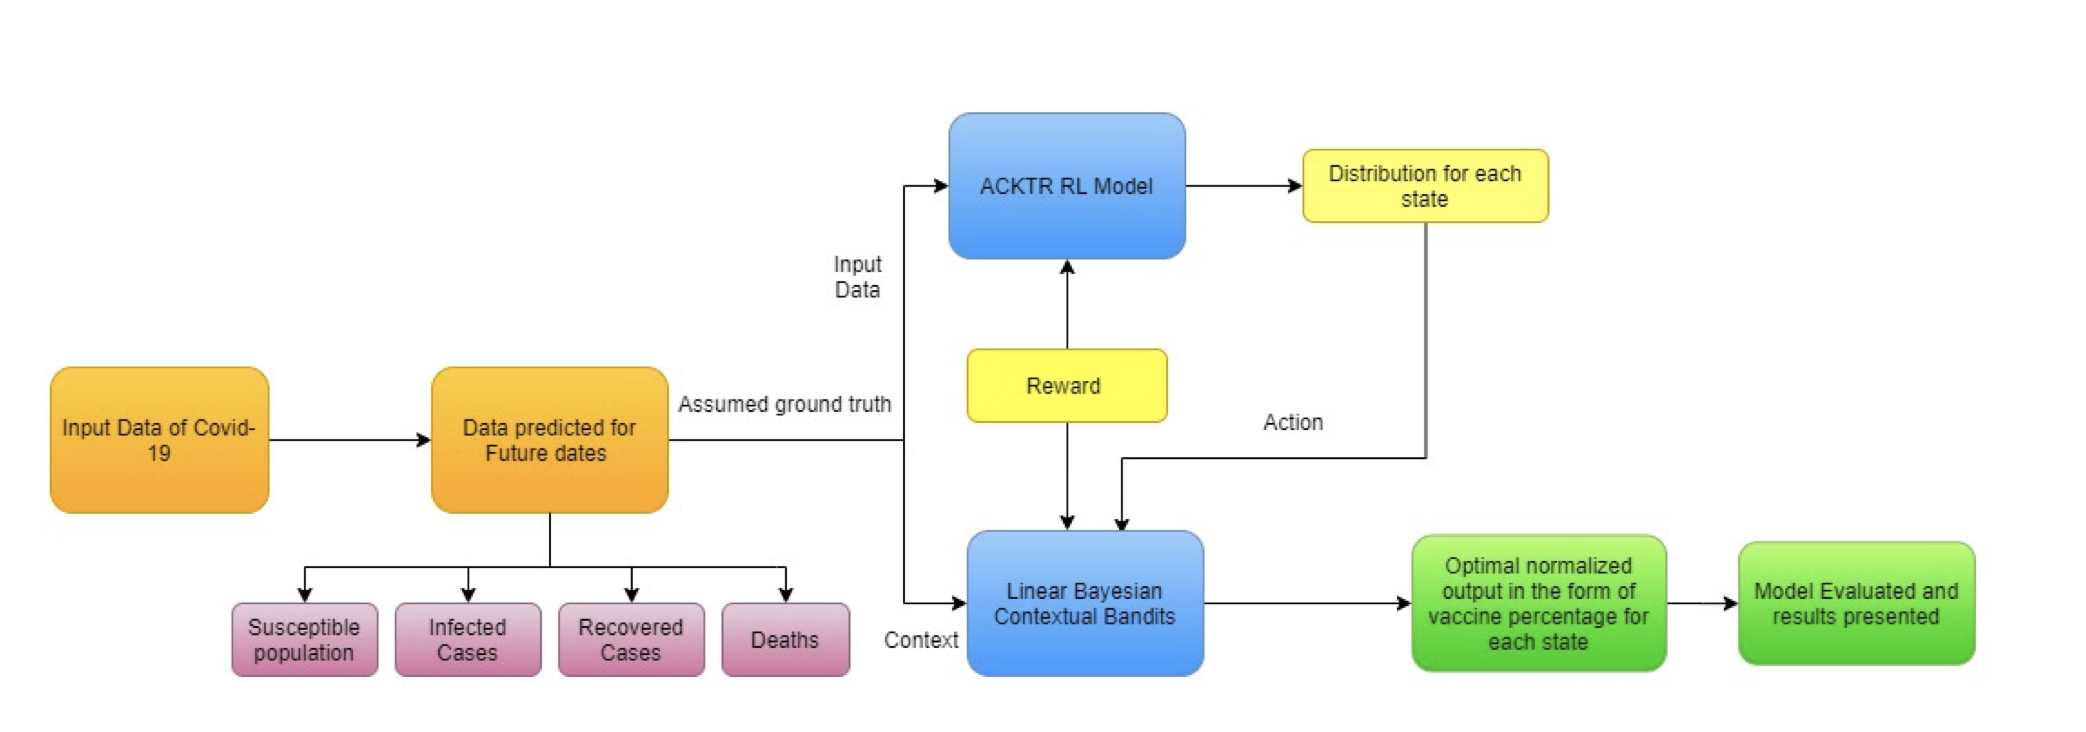
\includegraphics[width=\textwidth]{model.png}
	\item 

\end{enumerate} 
 

\section{Cold chain consideration}

Cold chain ie the storage method of vaccine on a minimum temperature range, vaccine are biological products that become ineffective over period of time, when exposed a loss of potency happen. There are various other reason for vaccine waste like in Delhi fewer people showing up as expected\footnote{https://www.hindustantimes.com/india-news/hesitancy-causes-wastage-of-1-000-vaccine-doses-in-delhi-say-health-officials-101611091051711.html}. On the delivery site there is only limited storage modes that does not last for long.

\subsection{Studies}

 14 and 35\% of refrigerators or transport shipments were found to have exposed vaccines to freezing temperatures, while in studies that examined all segments of distribution, between 75 and 100\% of the vaccine shipments were exposed.\cite{kartoglu2014tools}. Freezing occurs when vaccine in transit use ice packs for storage, other alternative is to use cold water packs. When developers and manufacturers are designing equipment to store vaccines at locations throughout the supply chain and during transport, there may be a tendency to focus on the individual user rather than the entire supply chain. But storage equipment sits within a larger ecosystem and characteristics such as power requirements, internal capacity, and price can have reverberating effects throughout the supply chain. Vaccine supply chain performance and efficiency depend on the ability of the system to meet storage device needs (such as maintenance technicians and spare parts) in the field. For example, the value of a passive vaccine storage device, i.e. ones that do not require a power source, depends on how well the ice supply chain can be coordinated, how mobile the device is, and how empty devices are swapped with refilled devices.\cite{lee2017importance}
 
  Currently available vaccines possess shortcomings, such as inefficient triggering of a cell-mediated immune response and the lack of protective mucosal immunity. In this regard, recent work has been focused on vaccine delivery systems, as an alternative to injectable vaccines, to increase antigen stability and improve overall immunogenicity. In particular, novel strategies based on edible or intradermal vaccine formulations have been demonstrated to trigger both a systemic and mucosal immune response. These novel vaccination delivery systems offer several advantages over the injectable preparations including self-administration, reduced cost, stability, and elimination of a cold chain \cite{criscuolo2019alternative}
 
 \subsection{Alternative Transformation}
 Nigeria was suffering from lowest vaccination rates in the world Taking end to end approach, Nigeria used strategy combining innovations in how data was captured, recorded and used to drive decision making and performing higher levels of uptime.\cite{sarley2017transforming}
 
 Methods like HERMES computational simulation model for on ground implementation like in case of Mozambique resulted in vaccine delivery to 27\% The alternative system also produced higher availability at lower costs after new vaccine introductions.\cite{LEE20164998}
 
 In some situations it is more efficient to bring the vaccines to the people instead of the other way around. Mobile medical teams need to route vaccines from one location to another. Halper and Raghavan define the mobile facility routing problem, with moving facilities to serve demand at different nodes in a network. In case of multiple facilities the routing problem is NP-hard and a heuristic is proposed to solve the problem.\cite{duijzer2018literature}
 
 Using constant data loggers as described above in the section of eventing layer, and data layer for synchronised behaviour across all domain. This helps in improving instant action and fall back strategies like what to do when a temperature falls below certain level.
 
 \subsection{Handling Waste}
 
 Design of the medical waste supply chain is critical for supplies that have been used for infectious patients, where the risk of further transmission is always imminent. Pishvaee et al. (2014) propose a method to design a sustainable medical supply chain, considering the complete life cycle of medical supplies and waste. Saif and Elhedhli (2016) take environmental considerations into account when studying the design of a cold supply chain. \cite{duijzer2018literature}
 
 \subsection{Integration}
 The WHO recommends integrating the vaccine supply chain with other health supply chains. Yadav et al. (2014) study the possibilities of integration. Outsourcing can be beneficial, although it is important to consult all stakeholders in advance, they say. These studies provide illustrations of successful integration from which lessons can be learnt. The authors conclude it is highly important to carefully determine which parts of the supply chain should be outsourced and to whom.\cite{duijzer2018literature}
 In India there are various methods like using public and private transport infrastructure for delivery methods, private companies like Uber, Ola has built technology that maps faster routes with maximum optimisation of delivery end to end. One use case like utilising existing fleet to transport vaccine internally in local region.
\section{Cryptographic Methods}

Data privacy while delevering vaccine is something that needs thorough though, a process that define how data is governed interanally and how its going to be shared with stakejolders. This data includes health records and constant monitoring of the users, crucial security is an important pillar in vaccine network. Govt system are highly centralised in nature , definelty a trade off of security 
	
\section{Challenges}

Recent studies indicate 71\% of individual from 19 countries would take vaccine. Countries like Russia where only 55\% are willing to participate in the excercise. Governments will have tough time ahead comvincing users. Gaining effectively trust government today needs to fundamentally shift its view and directly motivate citizens with the use of effective data driven planning and dialogue. Right now country like India where scientist from all across diferent domain are raising voices against the vaccine production and its efficacy since some vaccine did not even go to phase 3. 

\subsection{Transparency}

Vaccine builders and government have to be open and clear about the data that it provides to user.

\subsection{Building for Future}

Governemtn needs to start building platforms and system with thinking for future. Technology can be used where value driven systems are in place and citizens can access true information from governemtn abouth thier health.	
  


\bibliographystyle{aabbrv}
\bibliography{bib/graph}


\end{document}




